\documentclass[a4paper,12pt]{article}
\usepackage{amsmath,amssymb,amsfonts,amsthm}
\usepackage{tikz}
\usepackage [utf8] {inputenc}
\usepackage [T2A] {fontenc} 
\usepackage[russian]{babel}
% Так ссылки в PDF будут активны
\usepackage[unicode]{hyperref}
\usepackage{ textcomp }
\usepackage{indentfirst}


%===============================================================================

% Title settings for Russian language in amsart

%===============================================================================

\makeatletter
\def\@settitle{\begin{center}%
		\baselineskip14\p@\relax
		\bfseries\scshape
		\@title
	\end{center}%
}
\makeatother

%===============================================================================

% Theorem styles

%===============================================================================
\usepackage{amsxtra}
\usepackage{enumitem, fancyref, theoremref}
\usepackage{amsrefs, latexsym, pstricks, mathtext}
\usepackage{hyperref, caption, listings}

\hypersetup{
	colorlinks=true,
	linkcolor=blue,
	filecolor=magenta,      
	urlcolor=cyan,
	pdftitle={Overleaf Example},
	pdfpagemode=FullScreen,
}

\urlstyle{same}

\renewenvironment{proof}{{\bfseries\itshape Доказательство.}}{\begin{flushright}
		$\Box$
\end{flushright}}

\newenvironment{sol}{{\bfseries\itshape Решение.}}{\begin{flushright}
		$\Box$
\end{flushright}}

\theoremstyle{plain}
\newtheorem*{quest}{Вопрос}
\newtheorem{prop}{Предложение}
\newtheorem{theorem}{Теорема}[section]
\newtheorem{lemma}{Лемма}[section]

\theoremstyle{remark}
\newtheorem{conseq}{Вывод}
\newtheorem{rem}{Замечание}

\theoremstyle{definition}
\newtheorem{definition}{Определение}

\newtheoremstyle{problem}
{\topsep}   % ABOVESPACE
{\topsep}   % BELOWSPACE
{\normalfont}  % BODYFONT
{0pt}       % INDENT
{\bfseries} % HEADFONT
{.}         % HEADPUNCT
{5pt plus 1pt minus 1pt} % HEADSPACE
{}          % CUSTOM-HEAD-SPEC
\newtheorem{problem}{Задача}

%===============================================================================



% вы сможете вставлять картинки командой \includegraphics[width=0.7\textwidth]{ИМЯ ФАЙЛА}
% получается подключать, как минимум, файлы .pdf, .jpg, .png.
\usepackage{graphicx}
% Если вы хотите явно указать поля:
\usepackage[margin=1in]{geometry}
% Или если вы хотите задать поля менее явно (чем больше DIV, тем больше места под текст):
% \usepackage[DIV=10]{typearea}

\usepackage{fancyhdr}

\newcommand{\bbR}{\mathbb R}%теперь вместо длинной команды \mathbb R (множество вещественных чисел) можно писать короткую запись \bbR. Вместо \bbR вы можете вписать любую строчку букв, которая начинается с '\'.
\newcommand{\eps}{\varepsilon}
\newcommand{\bbN}{\mathbb N}
\newcommand{\dif}{\mathrm{d}}

\newtheorem{Def}{Definition}

%===============================================================================
%%%%%%%%%%%%%%%%%%%%%%%%%%%% Block schema %%%%%%%%%%%%%%%%%%%%%%%%%%%%%%%%%%%%%%
%===============================================================================

\usepackage{tikz}

\usetikzlibrary{shapes, arrows}

\tikzstyle{decision} = [
	diamond,
	draw,
	fill = green!20,
	text width = 6em,
	text badly centered,
	node distance = 2cm,
	inner sep = 0pt
]
\tikzstyle{block} = [
	rectangle,
	draw,
	fill = blue!20,
	text width = 8em,
	text centered,
	rounded corners,
	minimum height = 2em
]
\tikzstyle{line} = [
	draw,
	-latex'
]
\tikzstyle{cloud} = [
	draw,
	ellipse,
	fill = red!20,
	node distance = 3cm,
	minimum height = 2em
]

\tikzstyle{blanc} = [
		draw=white,
		rectangle,
		fill = white,
		minimum width = 0em,
		minimum height = 0em
]

%================================================================================

\usepackage{listings}

\lstset{
	language=C++,                 % выбор языка для подсветки 
	basicstyle=\small\ttfamily, % размер и начертание шрифта для подсветки кода
	keywordstyle=\color{blue},	% цвет ключевых слов
	commentstyle=\color[rgb]{0,0.5,0},	% цвет комментариев
	numbers=left,               % где поставить нумерацию строк (слева\справа)
	numberstyle=\tiny\color{gray},           % размер шрифта для номеров строк
	stepnumber=1,                   % размер шага между двумя номерами строк
	numbersep=5pt,                % как далеко отстоят номера строк от подсвечиваемого кода
	backgroundcolor=\color{white}, % цвет фона подсветки - используем \usepackage{color}
	showspaces=false,            % показывать или нет пробелы специальными отступами
	showstringspaces=false,      % показывать или нет пробелы в строках
	showtabs=false,             % показывать или нет табуляцию в строках
	frame=single,              % рисовать рамку вокруг кода
	tabsize=4,                 % размер табуляции по умолчанию равен 2 пробелам
	captionpos=t,              % позиция заголовка вверху [t] или внизу [b] 
	breaklines=true,           % автоматически переносить строки (да\нет)
	breakatwhitespace=false, % переносить строки только если есть пробел
	escapeinside={\%*}{*)},   % если нужно добавить комментарии в коде
	extendedchars=true
}

\lstset{tabsize=2,
	breaklines,
	columns=fullflexible,
	flexiblecolumns,
	numbers=left,
	numberstyle={\footnotesize},
	extendedchars=false,
	keepspaces=true
}

\pagestyle{fancy}
\makeatletter % сделать "@" "буквой", а не "спецсимволом" - можно использовать "служебные" команды, содержащие @ в названии
\fancyhead[L]{\footnotesize \@title}%Это будет написано вверху страницы слева
\fancyhead[R]{\footnotesize <<Физтех-лицей>> им. П. Л. Капицы}
\fancyfoot[L]{\footnotesize \@author}%имя автора будет написано внизу страницы слева
\fancyfoot[R]{\@date}%номер страницы —- внизу справа
\fancyfoot[C]{\thepage}%по центру внизу страницы пусто

\renewcommand{\maketitle}{%Настройка заголовка
	\noindent{\bfseries\scshape\large\@title\ \mdseries\upshape}\par
	\noindent {\large\itshape Author: \@author}
	\vskip 2ex}
\makeatother
\def\dd#1#2{\frac{\partial#1}{\partial#2}}
\def\ssum#1#2{\sum\limits_{#1}^{#2}}
\def\l{\langle}
\def\r{\rangle}

\graphicspath{{images//}}

\hypersetup{
	pdfauthor={Kim Zyong}
}

\usepackage{multirow}
\usepackage{colortbl}





\title{Отчёт по заданию к семинару 3\\Вариант 22}
\author{Ким Зыонг ИДз-22-20} 
\date{\today}

\begin{document}
	\maketitle
	
	\section{Условие задачи}
	
	Для каждой строки матрицы $A (4\times5)$ вычислить сумму и количество
	отрицательных элементов, а для каждой строки матрицы $B (3\times 7)$ — сумму и
	количество элементов, значения которых меньше 5.
	
	\section{Измененный функционал программы}
	
	Пользователь может задать размеры матрицы, а далее поэлементно менять её значение. Можно запросить сумму и количество элементов, меньших некоторого q, в каждой строке или во всей матрице. Результат появится в таблице справа от матрицы.
	
	\section{Материалы}
	
	Все материалы проекта доступны по ссылке: \url{https://github.com/KimonSenpai/OOP/tree/main/LAB-3}
	
	Основные файлы:
	\begin{enumerate}
		\item Lab-3 --- папка с проектом;
		
		\item Lab-3.pdf --- отчёт по работе;
		
		\item Lab-2.tex --- исходник данного документа.
	\end{enumerate}
	\section{Внесенные изменения}
	
	Ввиду того, что программа стала оконной, а не консольной, были удалены методы потокового ввода и вывода. Они заменены сеттером и геттером для элементов матрицы, а результат запросов просто возвращается из методов. Также хранение матрицы было переделано с векторов на List.
	
	\section{Обработчики событий}
	
	В программе 4 основных обработчика событий: нажатия на кнопки и задание значений матрицы.
	
	\begin{enumerate}
		\item Нажатие кнопки задания размеров создает матрицу (как внутреннее представление, так и отображает на форме). Изначально она содержит нули. В случае, если ввод был некорректным, выдается предупреждение и действие отменяется. Код обработчика событий:
		
		\begin{lstlisting}[language=C++]
private: System::Void SetSize_Click(System::Object^ sender, System::EventArgs^ e) {
	// Проверка правильности ввода данных
	try {
		m = Convert::ToInt32(SizeM->Text);
		n = Convert::ToInt32(SizeN->Text);
	}
	catch (...) {
		MessageBox::Show(L"Неправильные размеры!", L"Ошибка", MessageBoxButtons::OK, MessageBoxIcon::Error);
		
		return;
	}
	
	if (m <= 0 || n <= 0) {
		MessageBox::Show(L"Неправильные размеры!", L"Ошибка", MessageBoxButtons::OK, MessageBoxIcon::Error);
		return;
	}
	
	initMatrix = true;// Отключение события ValueChange у матрицы.
	Matrix->Rows->Clear();
	Matrix->Columns->Clear();
	
	Resoult->Rows->Clear();
	Resoult->Columns->Clear();
	
	
	
	matrix = gcnew ModifiedMatrix(m, n);
	
	Matrix->ColumnCount = n;
	
	for (int j = 0; j < n; ++j) {
		Matrix->Columns[j]->HeaderText = j.ToString();
		Matrix->Columns[j]->Width = 50;
	}
	
	Resoult->ColumnCount = 2;
	
	Resoult->Columns[0]->HeaderText = L"Сумма";
	Resoult->Columns[1]->HeaderText = L"Количество";
	
	Resoult->Columns[0]->Width = 87;
	Resoult->Columns[1]->Width = 87;
	
	for (int i = 0; i < m; ++i) {
		array<String^>^ row = gcnew array<String^>(n);
		for (int j = 0; j < n; ++j) {
			row[j] = "0";
		}
		Matrix->Rows->Add(row);
		Matrix->Rows[i]->HeaderCell->Value = i.ToString();
	}
	
	ByRow->Enabled = true;
	InMatrix->Enabled = true;
	initMatrix = false;// Включение события ValueChange у матрицы.
}
		\end{lstlisting}
		
		\item При изменении значения в матрице новое значение заносится и во внутреннее представление матрицы, если новое значение корректно. В ином случае выдается ошибка, а изменение откатывается. Код обработчика:
		
		\begin{lstlisting}[language=C++]
private: System::Void Matrix_CellValueChanged(System::Object^ sender, System::Windows::Forms::DataGridViewCellEventArgs^ e) {
	if (initMatrix) return;
	
	int i = e->RowIndex,
	j = e->ColumnIndex;
	
	// Проверка правильности ввода данных
	try {
		matrix->SetVal(i, j, Convert::ToInt32(Matrix->Rows[i]->Cells[j]->Value));
	}
	catch (...) {
		MessageBox::Show(L"Неправильное значение элемента матрицы!", L"Ошибка", MessageBoxButtons::OK, MessageBoxIcon::Error);
		Matrix->Rows[i]->Cells[j]->Value = matrix->GetVal(i, j).ToString();
	}
}
		\end{lstlisting}
		
		\item При построчном запросе вызывается метод ``CalcuateByRows'' у внутреннего представления матрицы. Результат вносится в таблицу. Если q было введено неправильно, выдается ошибка и никаких изменений не происходит. Код обработчика:
		
		\begin{lstlisting}[language=C++]
private: System::Void ByRowReq_Click(System::Object^ sender, System::EventArgs^ e) {
	int q;
	Resoult->Rows->Clear();
	
	// Проверка правильности ввода данных
	try {
		q = Convert::ToInt32(ByRowQ->Text);
	}
	catch (...) {
		MessageBox::Show(L"Неправильное значение q!", L"Ошибка", MessageBoxButtons::OK, MessageBoxIcon::Error);
		return;
	}
	
	auto res = matrix->CalculateByRows(q);
	
	for (int i = 0; i < res->Count; ++i) {
		array<String^>^ row = gcnew array<String^>(2);
		row[0] = res[i]->Item1.ToString();
		row[1] = res[i]->Item2.ToString();
		Resoult->Rows->Add(row);
	}
}
		\end{lstlisting}
		
		\item При запросе на всю матрицу вызывается метод ``CalcuateInMatrix'' у внутреннего представления матрицы. Результат вносится в таблицу. Если q было введено неправильно, выдается ошибка и никаких изменений не происходит. Код обработчика:
		
		\begin{lstlisting}[language=C++]
private: System::Void InMatrixReq_Click(System::Object^ sender, System::EventArgs^ e) {
	int q;
	Resoult->Rows->Clear();
	
	// Проверка правильности ввода данных
	try {
		q = Convert::ToInt32(InMatrixQ->Text);
	}
	catch (...) {
		MessageBox::Show(L"Неправильное значение q!", L"Ошибка", MessageBoxButtons::OK, MessageBoxIcon::Error);
		return;
	}
	
	auto res = matrix->CalculateInMatrix(q);
	
	array<String^>^ row = gcnew array<String^>(2);
	row[0] = res->Item1.ToString();
	row[1] = res->Item2.ToString();
	
	Resoult->Rows->Add(row);
}
		\end{lstlisting}
	\end{enumerate} 
	
	\pagebreak
	\section{Скриншоты приложения}
	
	\begin{figure}[h!]
		\centering
		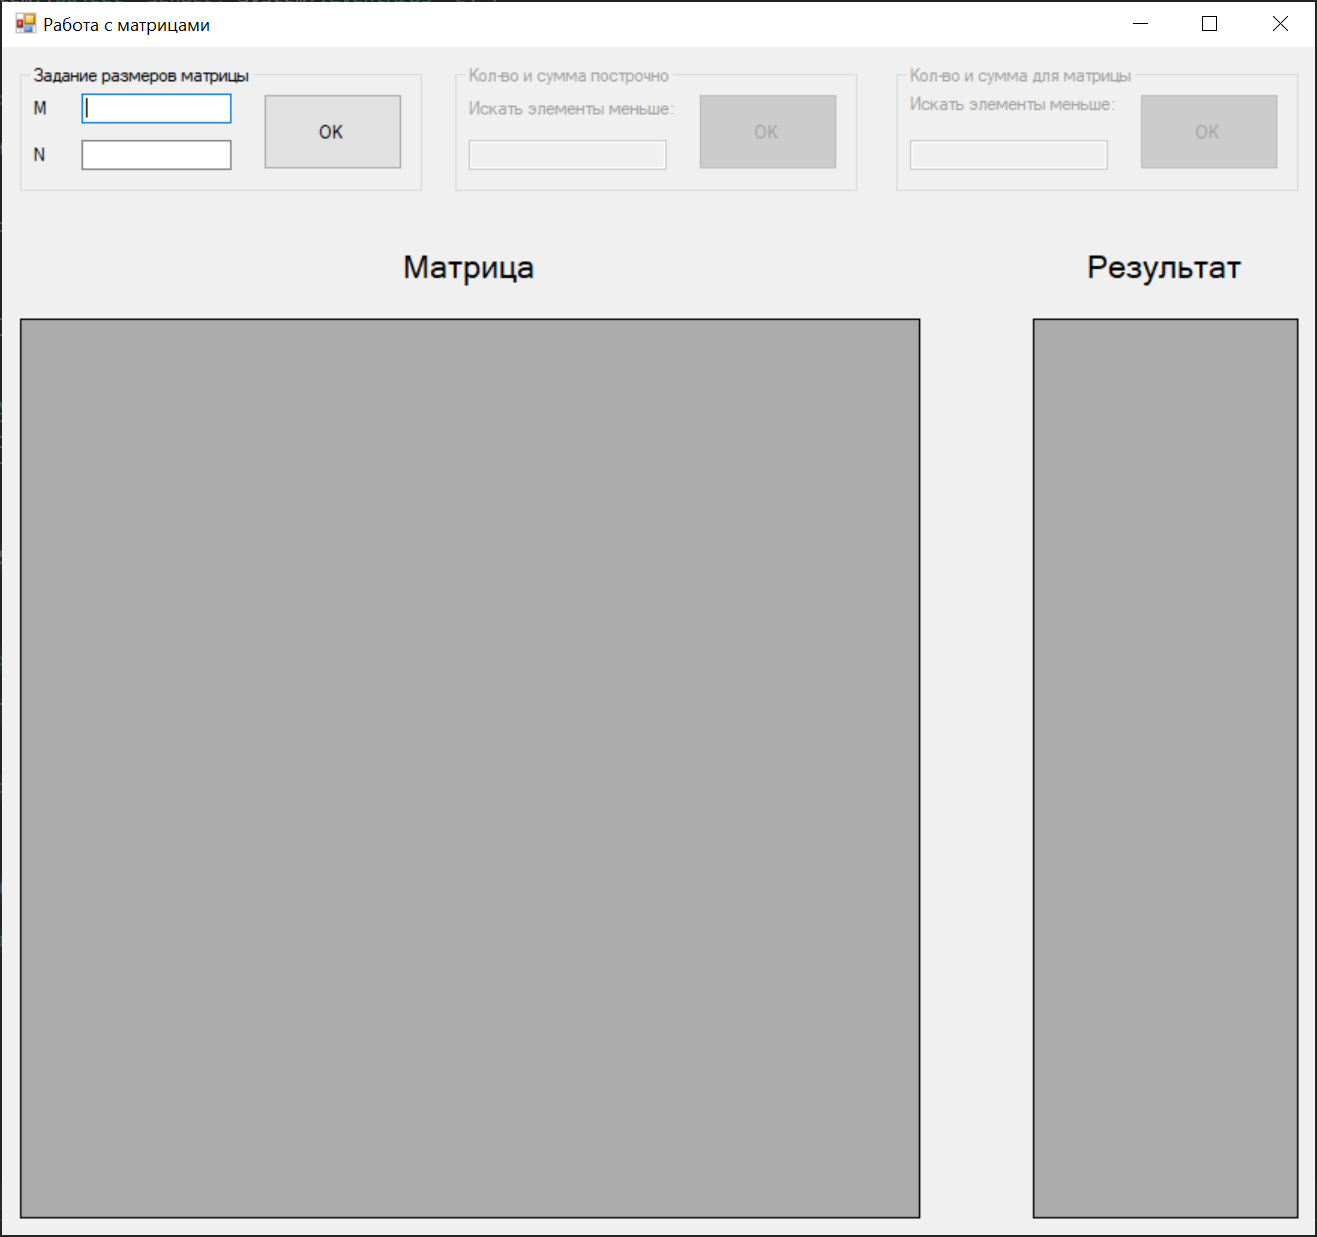
\includegraphics[width=.9\linewidth]{1.png}
		\caption{Вид при запуске.}
	\end{figure}
	
	\begin{figure}[h!]
		\centering
		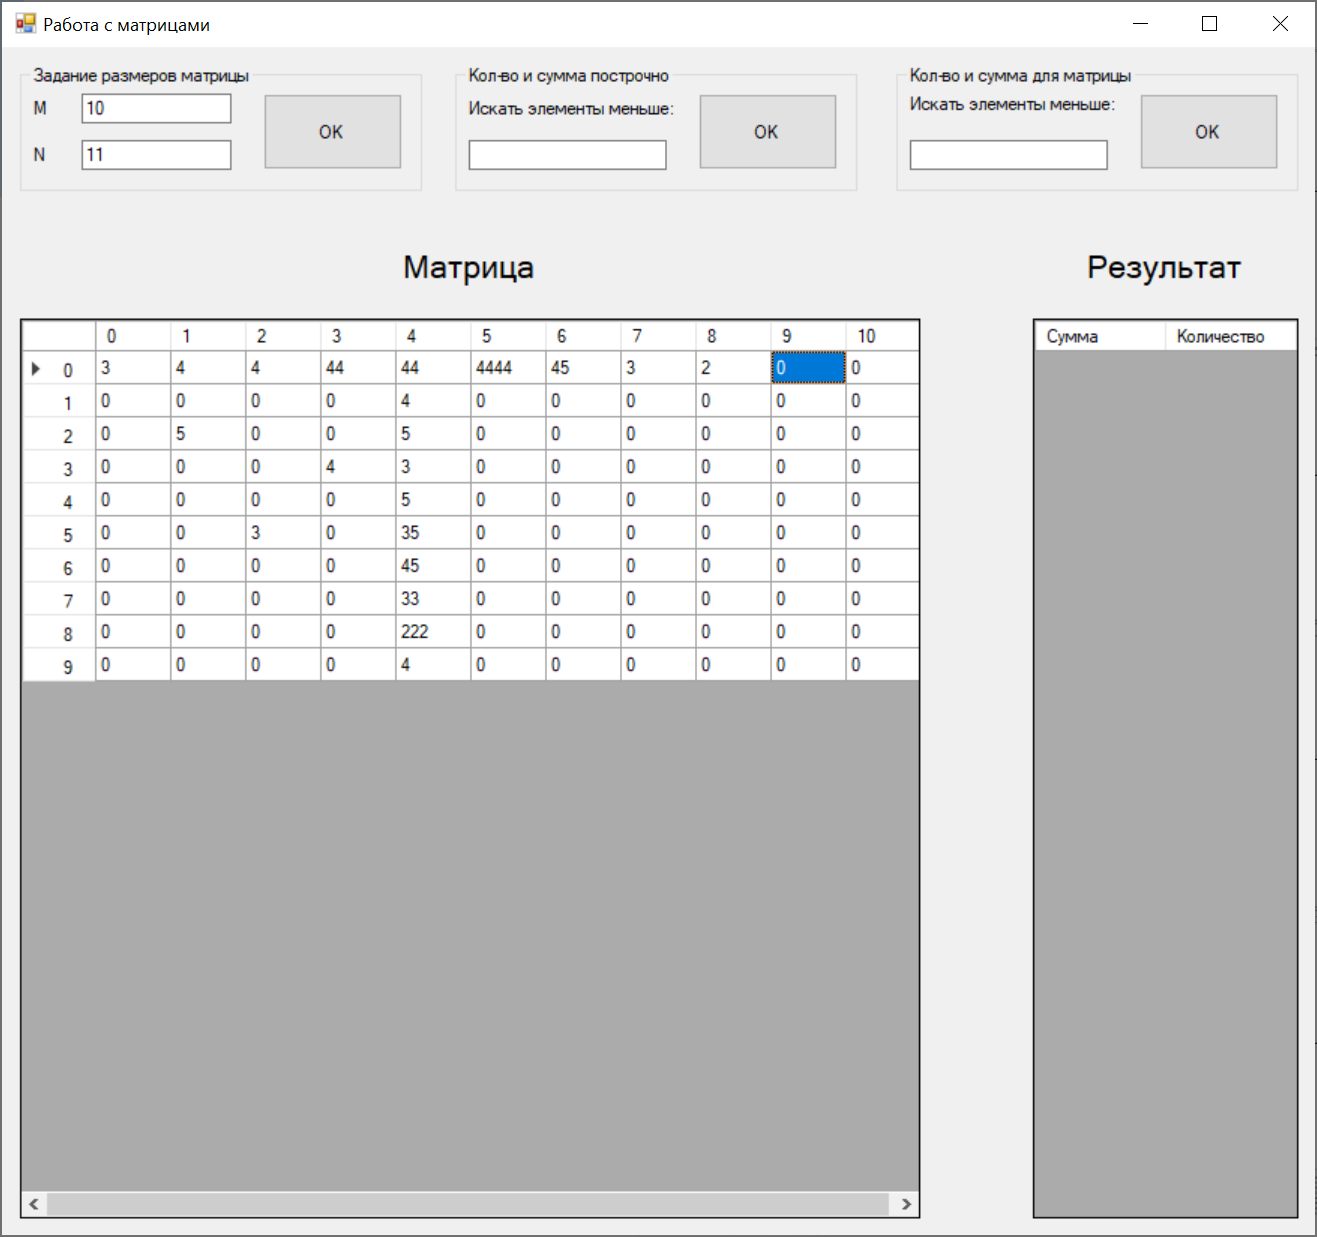
\includegraphics[width=.9\linewidth]{2.png}
		\caption{Ввод значений матрицы.}
	\end{figure}
	
	\begin{figure}[h!]
		\centering
		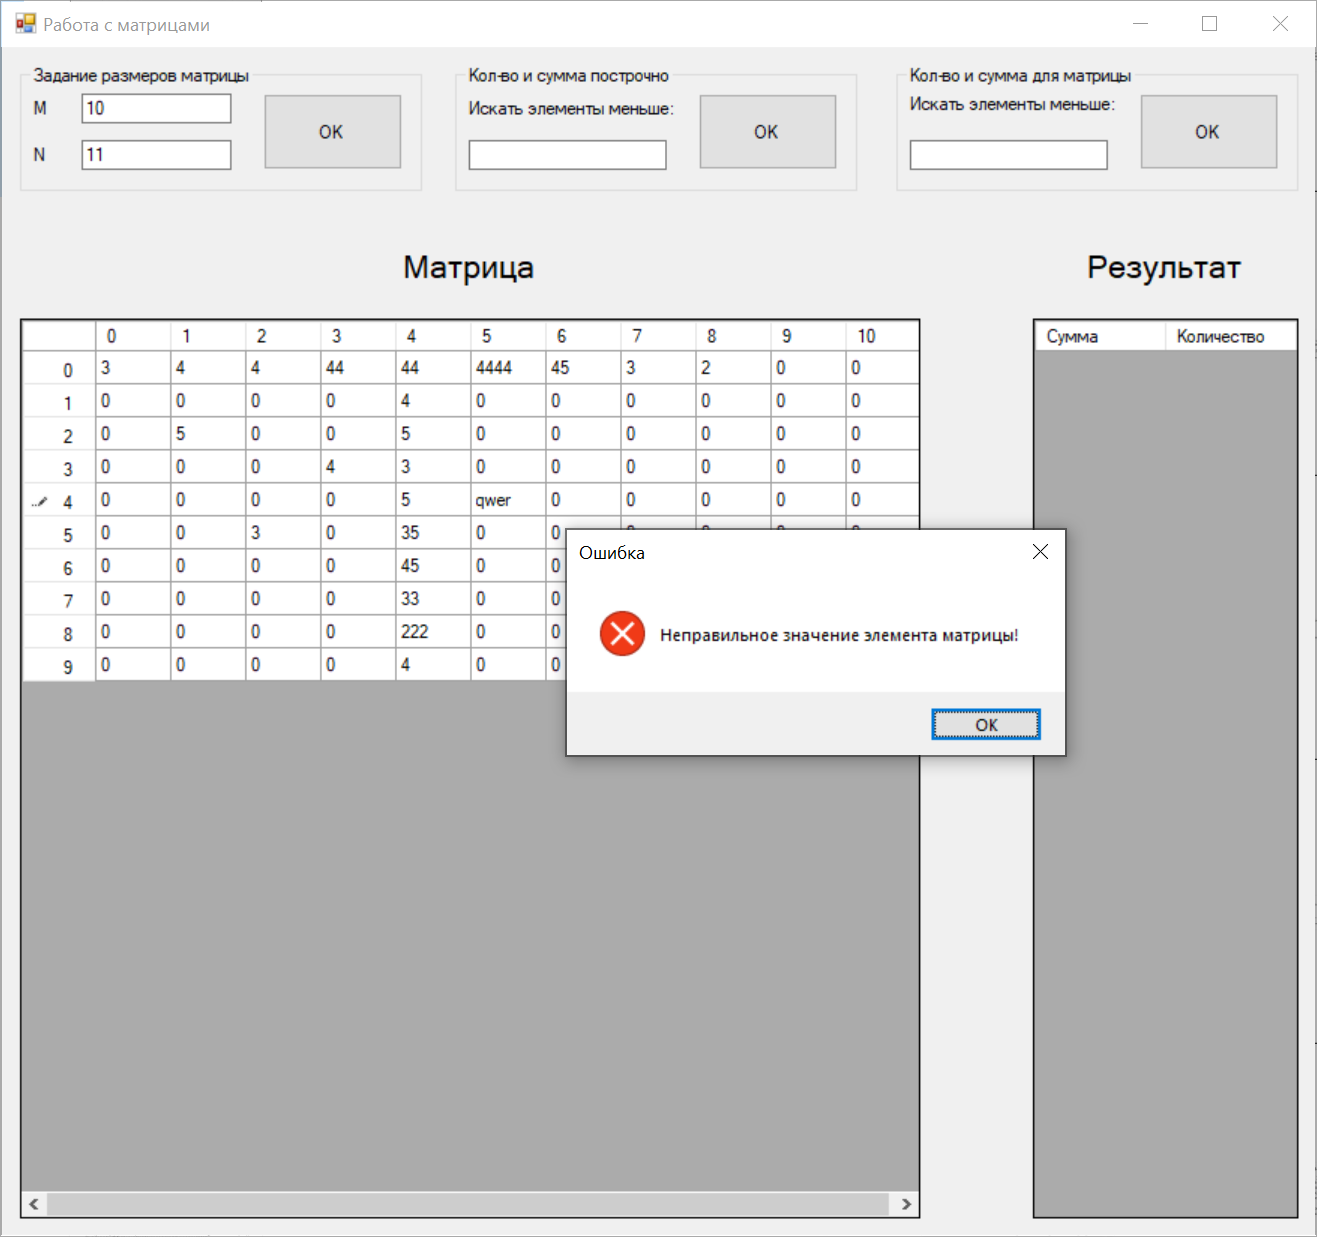
\includegraphics[width=.9\linewidth]{3.png}
		\caption{При некорректном вводе.}
	\end{figure}
	
	\begin{figure}[h!]
		\centering
		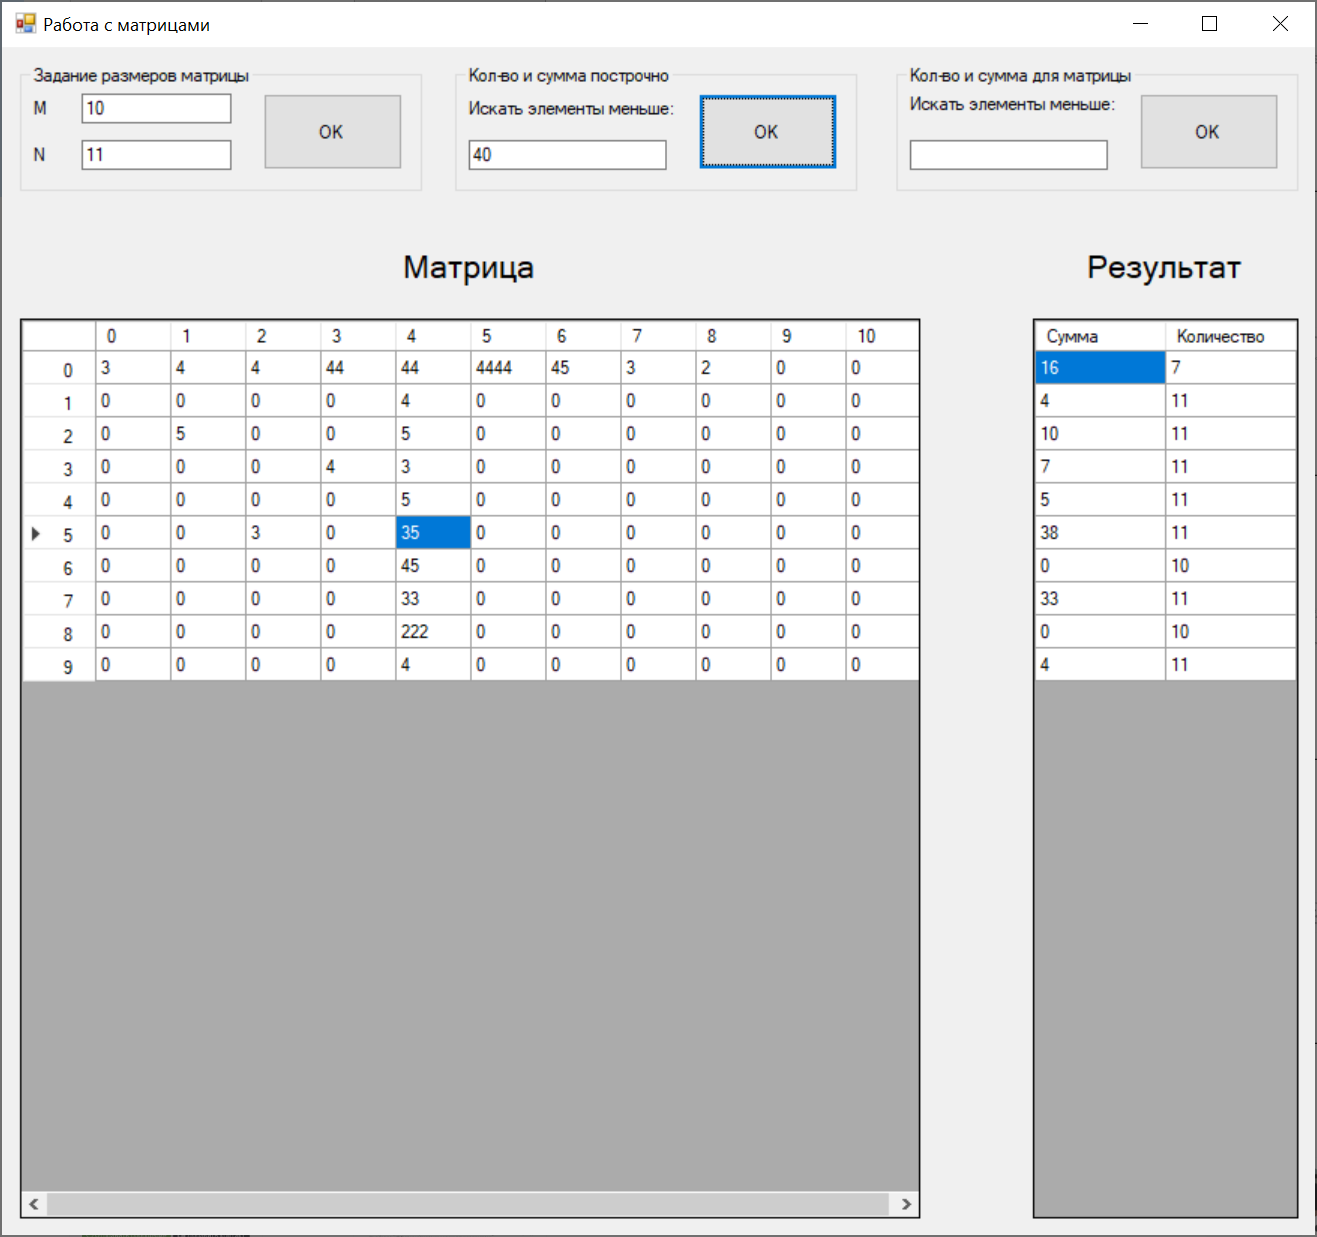
\includegraphics[width=.9\linewidth]{4.png}
		\caption{Результат построчного запроса.}
	\end{figure}
	
	\begin{figure}[h!]
		\centering
		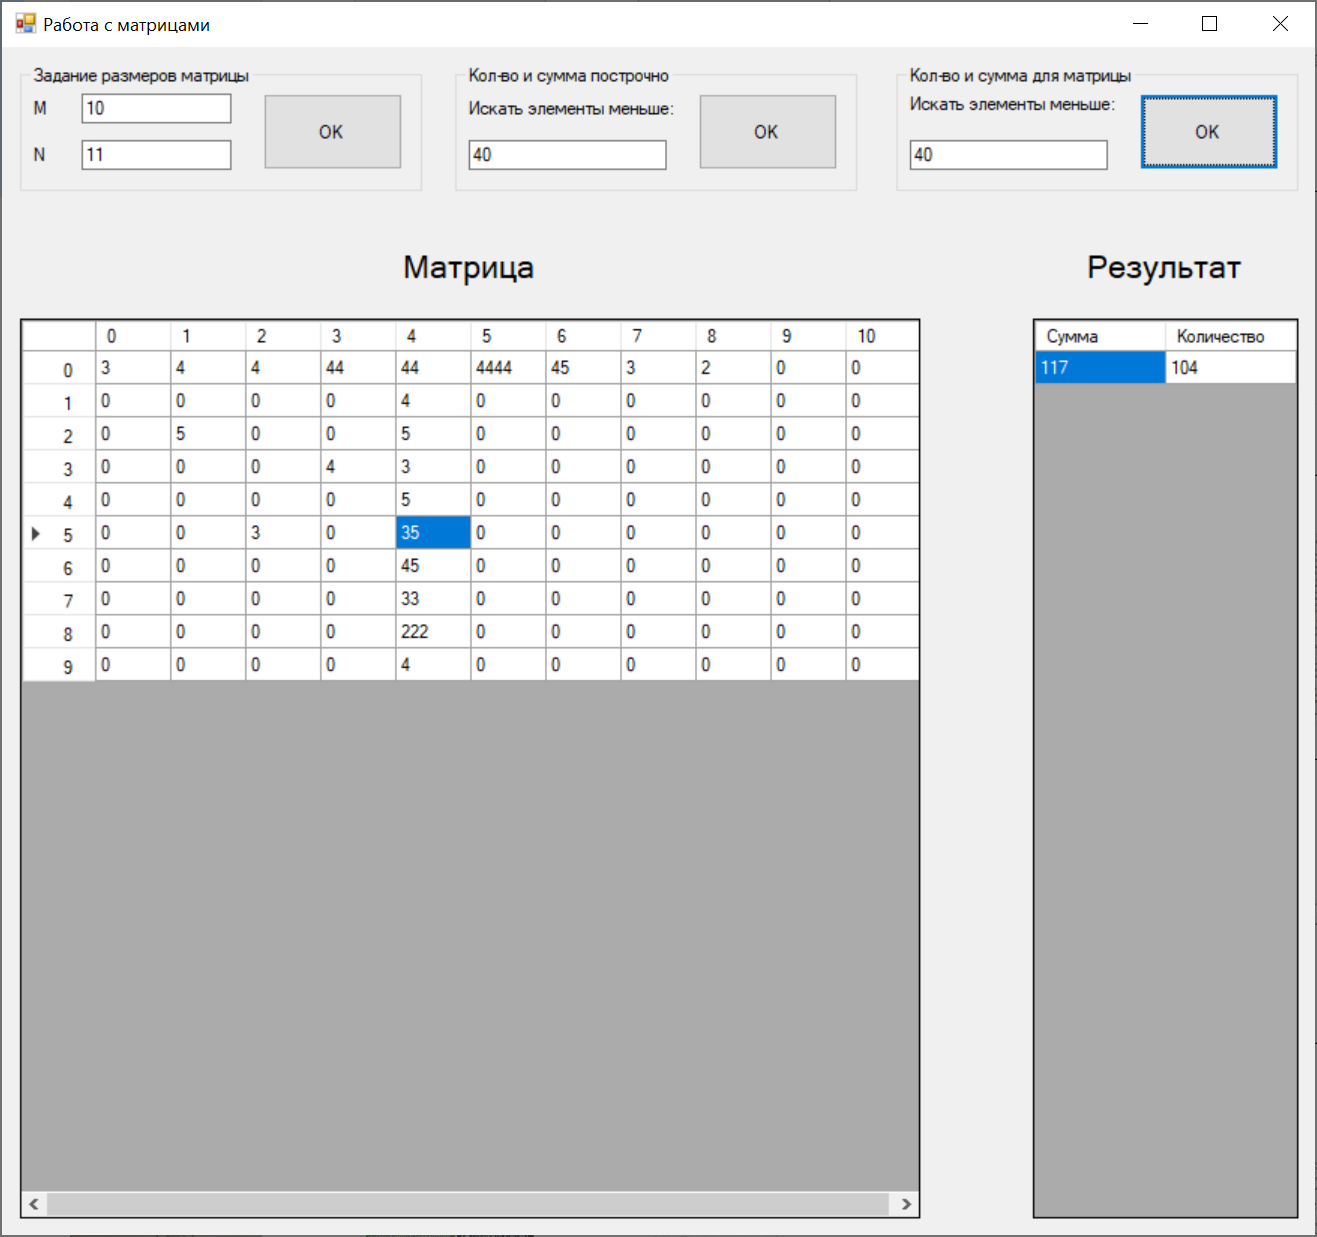
\includegraphics[width=.9\linewidth]{5.png}
		\caption{Результат запроса на всю матрицу.}
	\end{figure}
	
	\begin{figure}[h!]
		\centering
		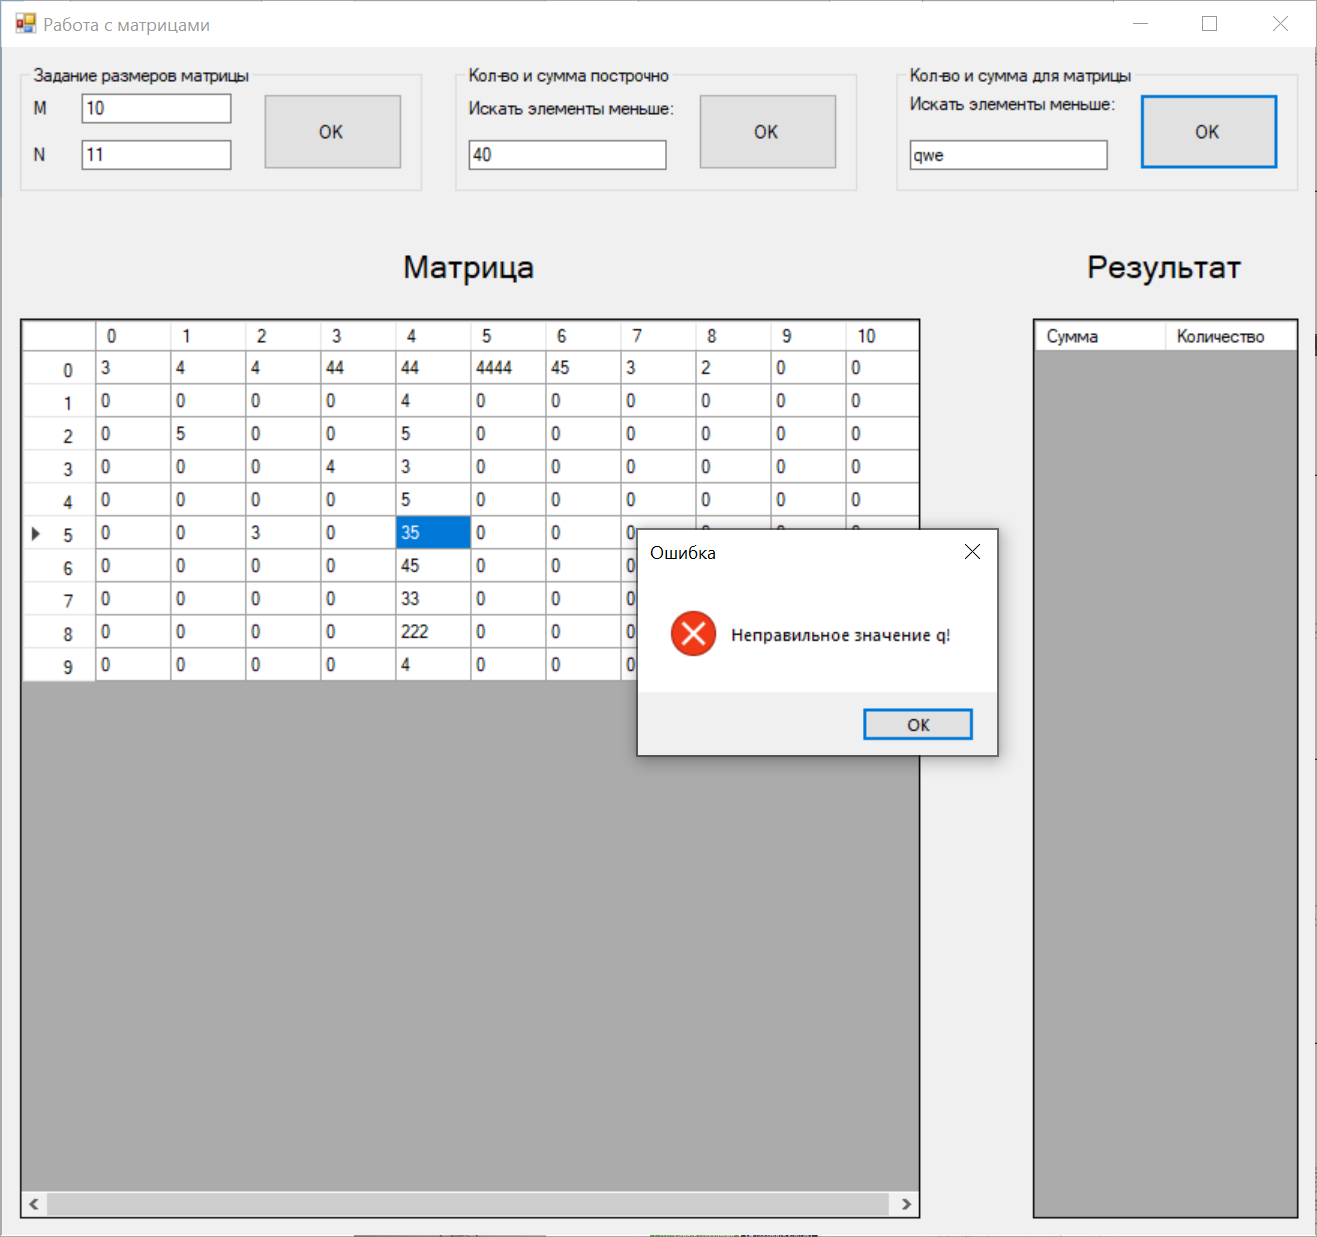
\includegraphics[width=.9\linewidth]{6.png}
		\caption{Некорректный ввод q.}
	\end{figure}
	
	
\end{document}